\section{Implement Neural Network Baselines}
I conducted two sets of experiments to compare gradient estimators with and
without baselines. The first (shown in \figref{baseline-small}) compares a
policy with and without baseline on the \texttt{InvertedPendulum-v1}
environment with a small batch size of 500 run on 5 seeds. The second (shown in
\figref{baseline-big}) compares a policy with baseline on the
\texttt{InvertedPendulum-v1} environment with a batch size of 10,000 against
the one shown in \figref{pendulum}. Both plots show that the estimators with
baselines perform comparably (sometimes slightly worse) to those without. The
baseline doesn't seem to help much on this task. The script used to run these
experiments is given in \figref{baseline-script}.

\begin{figure}[h]
  \centering
  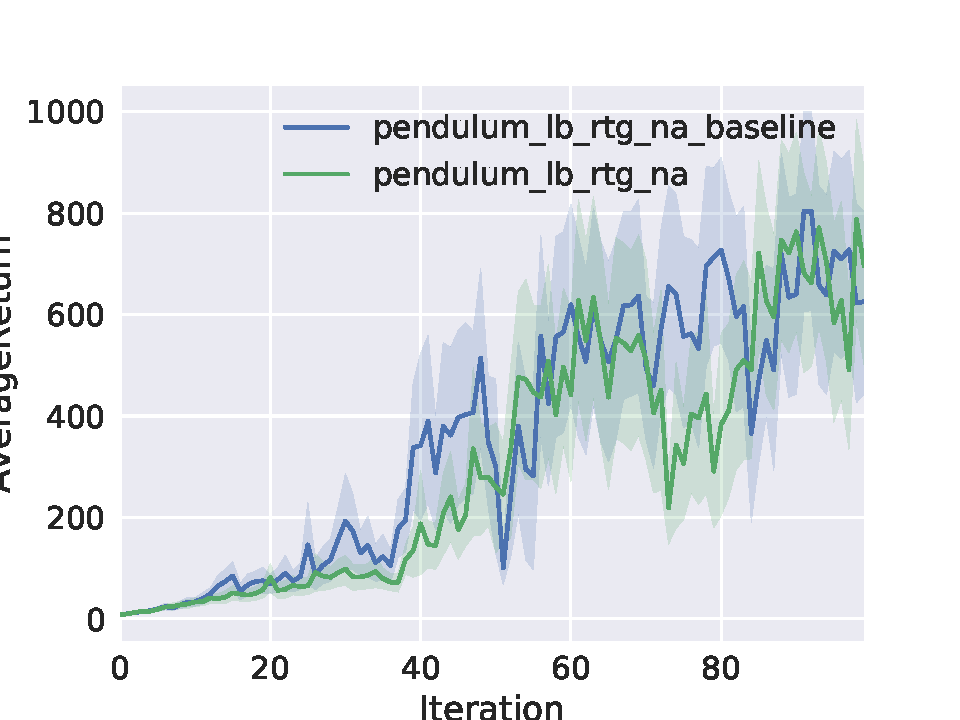
\includegraphics[width=\textwidth]{small_batch_pendulum_comparison.pdf}
  \caption{10,000 batch \texttt{InvertedPendulum-v1} baselines comparison.}
  \label{fig:baseline-small}
\end{figure}

\begin{figure}[h]
  \centering
  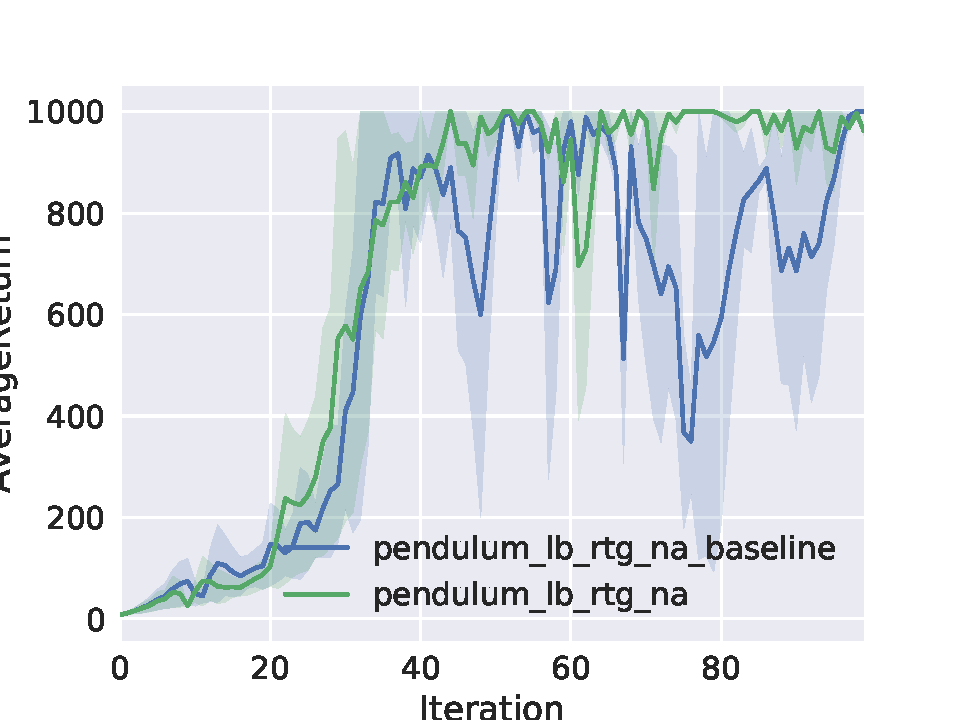
\includegraphics[width=\textwidth]{large_batch_pendulum_comparison.pdf}
  \caption{500 batch \texttt{InvertedPendulum-v1} baselines comparison.}
  \label{fig:baseline-big}
\end{figure}

\begin{figure}
  \centering
  \footnotesize
  \begin{Verbatim}[gobble=4]
    #! /usr/bin/env bash

    set -euo pipefail

    main() {
        python train_pg.py \
            InvertedPendulum-v1 \
            --verbose \
            --n_layers 2 \
            --size 32 \
            --seed 2 \
            -n 100 \
            -b 10000 \
            -e 5 \
            --discount 1 \
            --learning_rate 0.01 \
            -rtg \
            --nn_baseline \
            --baseline_batches 100 \
            --exp_name pendulum_lb_rtg_na_baseline

        python train_pg.py \
            InvertedPendulum-v1 \
            --verbose \
            --n_layers 2 \
            --size 32 \
            --seed 2 \
            -n 100 \
            -b 500 \
            -e 5 \
            --discount 1 \
            --learning_rate 0.005 \
            -rtg \
            --nn_baseline \
            --baseline_batches 100 \
            --exp_name pendulum_lb_rtg_na_baseline

        python train_pg.py \
            InvertedPendulum-v1 \
            --verbose \
            --n_layers 2 \
            --size 32 \
            --seed 2 \
            -n 100 \
            -b 500 \
            -e 5 \
            --discount 1 \
            --learning_rate 0.005 \
            -rtg \
            --exp_name pendulum_lb_rtg_na
    }

    main
  \end{Verbatim}
  \caption{Script use to run \texttt{InvertedPendulum-v1} baseline experiments.}
  \label{fig:baseline-script}
\end{figure}
